The frame M is a counterclockwise rotation of the global frame G by $\frac{\pi}{3}$ radians, and has its origin
at $(-3, 1)_G$

Draw the origin and basis vectors for frame G and frame M.

\begin{solution}\
\begin{center}
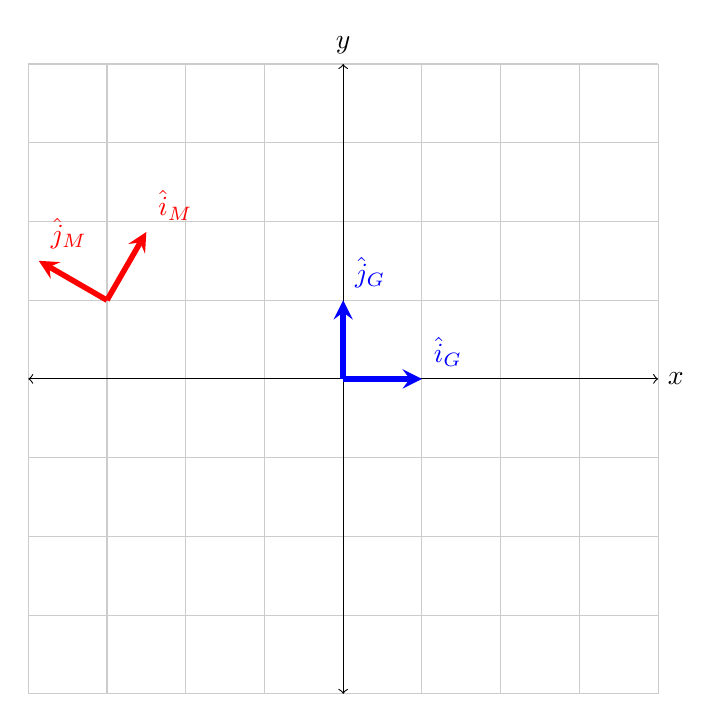
\begin{tikzpicture}
    \draw[thin,gray!40] (-4,-4) grid (4,4);
    \draw[<->] (-4,0)--(4,0) node[right]{$x$};
    \draw[<->] (0,-4)--(0,4) node[above]{$y$};
    \draw[line width=2pt,blue,-stealth](0,0)--(1,0) node[anchor=south west]{$\boldsymbol{\hat{i}}_G$};
    \draw[line width=2pt,blue,-stealth](0,0)--(0,1) node[anchor=south west]{$\boldsymbol{\hat{j}}_G$};
    \draw[line width=2pt,red,-stealth](-3,1)--(-2.5,1.866) node[anchor=south west]{$\boldsymbol{\hat{i}}_M$};
    \draw[line width=2pt,red,-stealth](-3,1)--(-3.866,1.5) node[anchor=south west]{$\boldsymbol{\hat{j}}_M$};
\end{tikzpicture}
\end{center}
\end{solution}